\documentclass[12pt,a4paper]{article}

% ==============================================================================
% SolarGuard AI - Informe Técnico y Académico (UNT - Sistemas Inteligentes)
% Documento actualizado progresivamente con métricas experimentales reales.
% ==============================================================================
\usepackage[utf8]{inputenc}
\usepackage[T1]{fontenc}
\usepackage[spanish,provide=*]{babel}
\usepackage{geometry}
\geometry{left=2.5cm,right=2.5cm,top=2.5cm,bottom=2.5cm}
\usepackage{graphicx}
\usepackage{booktabs}
\usepackage{longtable}
\usepackage{array}
\usepackage{float}
\usepackage{amsmath}
\usepackage{hyperref}
\usepackage{xcolor}
\usepackage{listings}
\usepackage{caption}
\usepackage{subcaption}

\definecolor{untblue}{HTML}{0E4D7A}
\definecolor{untgreen}{HTML}{1B6B46}
\definecolor{codebg}{HTML}{F6F8FA}

\hypersetup{
    colorlinks=true,
    linkcolor=untblue,
    citecolor=untgreen,
    urlcolor=untblue,
    pdftitle={SolarGuard AI - Informe Técnico Grupo 08},
    pdfauthor={Grupo 08 - UNT Sistemas Inteligentes}
}

\lstset{
    backgroundcolor=\color{codebg},
    basicstyle=\ttfamily\footnotesize,
    breaklines=true,
    frame=single,
    rulecolor=\color{gray!40}
}

\begin{document}

% ==============================================================================
% CARÁTULA
% ==============================================================================
\begin{titlepage}
    \centering
    \vspace*{1cm}
    {\Large \textbf{UNIVERSIDAD NACIONAL DE TRUJILLO}}\\[0.3cm]
    {\large FACULTAD DE INGENIERÍA}\\
    {\large ESCUELA PROFESIONAL DE INGENIERÍA DE SISTEMAS}\\[1.8cm]

    {\color{untblue}\rule{\linewidth}{1.5pt}}\\[0.5cm]
    {\LARGE \textbf{SolarGuard AI: Sistema Inteligente Híbrido para Inspección Visual y Pronóstico de Producción Fotovoltaica}}\\[0.3cm]
    {\large Arquitectura Mixture of Experts (MoE) Orquestada con LangGraph, Visión Computacional, Machine Learning Tabular y RAG Verificable}\\[0.2cm]
    {\color{untblue}\rule{\linewidth}{1.5pt}}\\[1.5cm]

    \begin{tabular}{ll}
        \textbf{Curso:} & Sistemas Inteligentes — VI Ciclo \\
        \textbf{Grupo:} & Grupo 08 \\
        \textbf{Área:} & Energías Renovables / Mantenimiento Predictivo \\
        \textbf{Semestre Académico:} & 2026-II \\
        \textbf{Modalidad:} & Proyecto Final Integrador (Backend, Modelos, RAG y Agente) \\
    \end{tabular}

    \vfill
    {\large Trujillo — Perú}\\
    {\large Noviembre de 2026}
\end{titlepage}

% ==============================================================================
% RESUMEN
% ==============================================================================
\begin{abstract}
\textbf{Resumen:} Este informe documenta el diseño, implementación y evaluación experimental del núcleo inteligente de \textbf{SolarGuard AI}, un sistema híbrido orientado a recomendar inspecciones técnicas en instalaciones fotovoltaicas mediante la integración de pronóstico de generación eléctrica, inspección visual multimodal (RGB y termografía infrarroja condicional) y asistencia documental verificable (RAG). Siguiendo la metodología CRISP-DM y el patrón \textit{Mixture of Experts} (MoE) orquestado sobre \textbf{LangGraph}, el sistema coordina cuatro expertos especializados bajo estrictas políticas anti-fuga, telemetría con registro diario coloreado y controles de seguridad (\textit{guardrails} anti-\textit{prompt injection} e intervención humana \textit{Human-in-the-Loop}). Experimentalmente, el predictor tabular \texttt{GradientBoostingRegressor} redujo el MAE en prueba temporal intacta de 23.266~kWh (baseline lineal) a 16.867~kWh (nMAE = 1.421\%); el clasificador RGB \texttt{MobileNetV3-Small} deduplicado por \texttt{pHash} logró Macro-F1 = 0.8276 (Recall = 0.9333 en grietas); el módulo térmico IR alcanzó Macro-F1 = 0.8731; el detector \texttt{YOLOv8n} obtuvo mAP@50 = 0.7580; y el motor RAG con \textit{guardrails} logró 100\% de \textit{Recall@3}, 90\% de exactitud de cita por página y 100\% de bloqueo adversarial en un banco de 20 consultas, integrándose en flujos LangGraph con latencia promedio de 194.5~ms por escenario.

\medskip
\noindent\textbf{Palabras clave:} Energía fotovoltaica, Mixture of Experts, LangGraph, Regresión tabular, Visión computacional, YOLOv8, MobileNetV3, Retrieval-Augmented Generation, Human-in-the-Loop.
\end{abstract}

\tableofcontents
\listoffigures
\listoftables
\newpage

% ==============================================================================
% I. INTRODUCCIÓN
% ==============================================================================
\section{Introducción}

\subsection{Contexto y realidad problemática}
La generación de energía eléctrica mediante sistemas solares fotovoltaicos (FV) exhibe una alta sensibilidad frente a variables meteorológicas dinámicas —principalmente irradiancia solar, temperatura ambiente y temperatura de módulo— así como frente a degradaciones superficiales o físicas (acumulación de polvo, excrementos de aves, sombreado parcial, fracturas del vidrio protector o fallos térmicos localizados). Según reportes de operación y mantenimiento (O\&M) de sistemas fotovoltaicos del \textit{National Renewable Energy Laboratory} (NREL, 2018), el ensuciamiento (\textit{soiling}) y las fallas no detectadas de módulos o cadenas pueden provocar pérdidas anuales de rendimiento energético significativas —que en entornos áridos o con baja frecuencia de limpieza superan habitualmente el 5\%–15\% e incluso alcanzan mermas mayores ante eventos puntuales—, mientras que las inspecciones visuales manuales periódicas suelen ejecutarse sin correlación directa con las series temporales de generación real.

En la práctica operativa tradicional, los monitores de inversores reportan caídas de potencia sin discriminar entre una reducción esperada por menor irradiancia y una anomalía atribuible al estado físico del panel. Inversamente, las rondas de inspección visual carecen de priorización cuantitativa basada en telemetría energética y no vinculan automáticamente el hallazgo visual con los protocolos técnicos normativos (como la norma IEC 62446 o guías de mantenimiento preventivo).

\subsection{Pregunta de investigación y justificación}
\textbf{Pregunta guía:} \textit{¿Cómo relacionar pronósticos de generación eléctrica e inspección visual multimodal para identificar paneles fotovoltaicos que merecen revisión técnica, respaldando cada recomendación con evidencia documental verificable y control humano?}

Una solución híbrida aporta valor tangible frente a la práctica manual porque: (1) normaliza la generación observada contra una línea base meteorológica para disparar alertas solo cuando la discrepancia excede un umbral operativo ($\geq 15\%$); (2) automatiza el cribado visual diferenciando paneles limpios, sucios, agrietados o con tomas no evaluables; (3) incorpora termografía infrarroja únicamente cuando se dispone de captura térmica; y (4) obliga a que toda recomendación de revisión esté sustentada en manuales técnicos con citas verificables y aprobación explícita de un técnico humano.

\subsection{Alcance, delimitaciones y riesgos}
El presente trabajo implementa la arquitectura completa de backend inteligente de \textbf{SolarGuard AI} (preparación anti-fuga de datos, entrenamiento y evaluación de modelos ML y CV, motor RAG con \textit{guardrails}, agente LangGraph con \textit{Human-in-the-Loop}, telemetría y pruebas automatizadas), excluyendo deliberadamente la interfaz gráfica en Streamlit. Como restricción ética y operativa estricta, el sistema \textbf{no emite comandos de desconexión eléctrica automatizada} ni diagnostica fallos eléctricos internos únicamente a partir de fotografías RGB.

% ==============================================================================
% II. ANTECEDENTES Y BASES TEÓRICAS
% ==============================================================================
\section{Antecedentes y Bases Teóricas}

\subsection{Antecedentes científicos}
En la Tabla~\ref{tab:antecedentes} se sintetizan seis trabajos científicos y técnicos verificables que fundamentan las dimensiones tabular, visual, termográfica y documental/agéntica de SolarGuard AI.

\begin{table}[H]
\centering
\caption{Matriz comparativa de antecedentes científicos verificables.}
\label{tab:antecedentes}
\scriptsize
\begin{tabular}{p{2.5cm}p{2.3cm}p{2.8cm}p{2.5cm}p{3.6cm}}
\toprule
\textbf{Referencia} & \textbf{Problema} & \textbf{Datos / Dominio} & \textbf{Técnicas / Métricas} & \textbf{Brecha / Aporte a SolarGuard AI} \\
\midrule
Khandakar et al. (2019) & Predicción de potencia FV & Series meteorológicas y generación FV & ANN, regresión; RMSE y MAE & No integra inspección visual ni protocolos de mantenimiento. \\
Mehta et al. (2018) & Detección de suciedad en paneles FV & Imágenes RGB de paneles solares & CNN (DeepSolarEye); exactitud y localización & Carece de enlace con telemetría eléctrica de planta. \\
Millendorf et al. (2020) & Clasificación de anomalías térmicas FV & Dataset \textit{InfraredSolarModules} (Raptor Maps) & CNN sobre parches IR; F1 por clase & Limitado a termografía aérea; requiere orquestación condicional. \\
Redmon et al. / Ultralytics (2023) & Detección de objetos en tiempo real & Imágenes aéreas y terrestres de paneles & YOLOv8; mAP@50 & Solo localiza paneles; requiere clasificador fino de daños. \\
Lewis et al. (2020) & Respuestas fundamentadas en corpus & Tareas intensivas en conocimiento & RAG (Dense Retrieval + Seq2Seq) & Base para citas verificables sin alucinaciones en manuales O\&M. \\
NIST (2024) & Gestión de riesgos en IA Generativa & Aplicaciones con LLM y agentes & Marco NIST AI 600-1 & Exige mitigación de \textit{prompt injection} y supervisión humana. \\
\bottomrule
\end{tabular}
\end{table}

\subsection{Bases teóricas}
\begin{itemize}
    \item \textbf{Patrón Mixture of Experts (MoE) Orquestado:} A diferencia de un MoE denso a nivel de capas neuronales, SolarGuard AI implementa un MoE funcional donde \textbf{LangGraph} actúa como red compuerta (\textit{Router / Gating Network}) que invoca selectivamente expertos especializados independientes según la evidencia disponible en el estado tipado \texttt{SolarGuardState}.
    \item \textbf{Aprendizaje Supervisado Libre de Fugas (\textit{No Data Leakage}):} En series temporales energéticas, el muestreo aleatorio mezcla observaciones autocorrelacionadas de un mismo día entre entrenamiento y prueba. Se exige partición temporal estricta por días consecutivos y encapsulamiento de imputación/escalado en \texttt{Pipeline}/\texttt{ColumnTransformer}. En visión artificial, imágenes aumentadas o capturadas en ráfaga sobre el mismo panel se agrupan mediante \textit{Perceptual Hashing} (\texttt{pHash}) antes de dividir conjuntos.
    \item \textbf{Retrieval-Augmented Generation (RAG) y Seguridad Documental:} El texto recuperado de manuales técnicos se trata exclusivamente como datos pasivos con trazabilidad de fuente y página, aplicando defensas contra inyección de instrucciones (\textit{prompt injection}) y detección explícita de ausencia de respaldo documental.
\end{itemize}

% ==============================================================================
% III. OBJETIVOS
% ==============================================================================
\section{Objetivos del Proyecto}

\subsection{Objetivo general}
Diseñar, implementar y evaluar el sistema inteligente integrado \textbf{SolarGuard AI} para recomendar inspecciones técnicas fotovoltaicas orientadas por discrepancias de generación, articulando modelos tabulares de Machine Learning, visión computacional (RGB, detección espacial YOLO y termografía condicional IR), recuperación documental verificable (RAG) y orquestación agéntica con control humano en LangGraph.

\subsection{Objetivos específicos}
\begin{enumerate}
    \item Construir una infraestructura reproducible con registro diario de eventos (\texttt{.log}), salida coloreada en \texttt{stdout} y telemetría de latencia y memoria.
    \item Preparar y modelar series temporales de generación eléctrica libre de fugas temporales, comparando una línea base lineal frente a modelos de ensamble mediante MAE, RMSE, nMAE y nRMSE.
    \item Desarrollar el componente de visión RGB de 4 clases con deduplicación perceptual (\texttt{pHash}), extensión espacial de detección de paneles (YOLO) y clasificador termográfico condicional (IR), medidos con Macro-F1, Recall de daños y mAP@50.
    \item Construir un sistema RAG verificable con citas de documento/página, defensas contra \textit{prompt injection} y benchmark de 20 consultas comparando \textit{Sin RAG} frente a \textit{Con RAG}.
    \item Orquestar todos los expertos en un grafo tipado de LangGraph con enrutamiento condicional, parada por incertidumbre, punto de intervención humana (\textit{Human-in-the-Loop}) y pruebas automatizadas con \texttt{pytest}.
\end{enumerate}

% ==============================================================================
% IV. METODOLOGÍA (CRISP-DM + INGENIERÍA DE SOFTWARE)
% ==============================================================================
\section{Metodología de Desarrollo}

El proyecto sigue la metodología \textbf{CRISP-DM} complementada con prácticas iterativas de ingeniería de software:

\begin{enumerate}
    \item \textbf{Comprensión del negocio:} Definición de reglas operativas (umbral de discrepancia energética del 15\%, umbral de confianza visual de 0.60 y prohibición de desconexión automatizada).
    \item \textbf{Comprensión y preparación de datos:} Auditoría de los cuatro datasets reales disponibles en \texttt{datasets/}, estandarización de formatos de fecha, agregación horaria, mapeo canónico de etiquetas y particiones estrictamente libres de fugas.
    \item \textbf{Modelado secuencial controlado:} Entrenamiento secuencial (un modelo/red a la vez, con límite de 4 hilos de CPU) para garantizar estabilidad de cómputo en entorno local sin GPU.
    \item \textbf{Evaluación integral:} Validación en conjuntos de prueba disjuntos e intactos, matriz de confusión, análisis de casos difíciles, benchmark RAG de 20 preguntas y verificación end-to-end del grafo LangGraph.
\end{enumerate}

% ==============================================================================
% V. IMPLEMENTACIÓN DE LA ARQUITECTURA
% ==============================================================================
\section{Implementación de la Arquitectura}

\subsection{Estructura modular y telemetría}
El código fuente se organiza bajo \texttt{src/} en seis paquetes cohesivos:
\begin{itemize}
    \item \texttt{src/core/}: configuración global (\texttt{config.py}), logging dual coloreado en \texttt{stdout} y archivo diario plano en \texttt{logs/solarguard\_YYYY-MM-DD.log} (\texttt{logging\_config.py}), y telemetría de eventos (\texttt{telemetry.py}).
    \item \texttt{src/data/}: pipelines reproducibles de limpieza, deduplicación perceptual y partición anti-fuga.
    \item \texttt{src/ml/}: entrenamiento e inferencia de regresión horaria tabular (\texttt{energia\_kwh\_hora}).
    \item \texttt{src/vision/}: clasificador RGB (4 clases), clasificador térmico IR condicional (3 clases), detector espacial YOLOv8n y módulo unificado de inferencia.
    \item \texttt{src/rag/}: constructor del corpus técnico paginado, almacén vectorial persistente, recuperador con umbral de evidencia, \textit{guardrails} de seguridad y evaluador benchmark.
    \item \texttt{src/agents/}: estado tipado \texttt{SolarGuardState}, esquemas Pydantic, 4 herramientas ejecutables, grafo MoE en LangGraph con \texttt{interrupt\_before=["validar\_tecnico"]} y ejecutor CLI de escenarios.
\end{itemize}

\subsection{Flujo de orquestación MoE en LangGraph}
El grafo implementa las siguientes rutas condicionales explícitas:
\begin{enumerate}
    \item \texttt{validar\_entradas}: valida rangos físicos (irradiancia $\geq 0$, capacidad $> 0$) e integridad de rutas de imagen. Ante fallos deriva a \texttt{manejar\_error}.
    \item \texttt{predecir\_energia}: calcula \texttt{expected\_energy\_kwh}, incertidumbre y \texttt{energy\_discrepancy\_pct}.
    \item \textbf{Router Condicional 1 (\texttt{evaluar\_discrepancia}):} si la discrepancia es $< 15\%$ y no se adjunta imagen ni inspección forzada, genera reporte normal (\texttt{redactar\_reporte\_normal}); en caso contrario invoca \texttt{detectar\_y\_clasificar\_rgb}.
    \item \textbf{Router Condicional 2 (\texttt{evaluar\_confianza\_y\_termica}):} si la etiqueta RGB es \texttt{vista no evaluable} o la confianza es $< 0.60$, activa \texttt{uncertainty\_flag = True} y detiene el diagnóstico solicitando nueva captura (\texttt{detener\_por\_incertidumbre}). Si la captura es evaluable y existe imagen térmica, ejecuta \texttt{clasificar\_termografia} antes de \texttt{consultar\_rag}.
    \item \texttt{generar\_propuesta\_revision} y \texttt{validar\_tecnico}: sintetiza el reporte Pydantic con citas verificables y pausa el grafo antes de emitir la orden simulada (\texttt{simular\_orden\_revision}) hasta recibir aprobación humana.
\end{enumerate}

% ==============================================================================
% VI. RESULTADOS EXPERIMENTALES Y DISCUSIÓN
% ==============================================================================
\section{Resultados Experimentales y Discusión}

\textit{Nota de actualización progresiva: las subsecciones siguientes se completan con las métricas y gráficas exactas obtenidas tras la ejecución de cada módulo.}

\subsection{Resultados del Experto 1: Módulo Tabular (Regresión de \texttt{energia\_kwh\_hora})}
\label{sec:res_tabular}
A partir de \texttt{Plant\_1\_Generation\_Data.csv} (68,778 lecturas) y \texttt{Plant\_1\_Weather\_Sensor\_Data.csv} (3,182 lecturas), se consolidaron 17,300 observaciones horarias válidas correspondientes a 22 inversores durante 34 días consecutivos (15 de mayo al 17 de junio de 2020). Se aplicó una partición temporal estricta sin mezcla aleatoria: Días 1--24 para entrenamiento (12,020 filas), Días 25--29 para validación (2,640 filas) y Días 30--34 para prueba intacta (2,640 filas). La capacidad instalada por inversor se calculó exclusivamente con el percentil 99 del conjunto de entrenamiento (mediana de referencia: 1,191.07~kWh/h).

La Tabla~\ref{tab:res_tabular} resume las métricas obtenidas en entrenamiento, validación y prueba. El modelo \textbf{GradientBoostingRegressor} (tasa de aprendizaje 0.05, profundidad máxima 3, 200 estimadores) obtuvo el menor RMSE en validación (30.603~kWh) y generalizó mejor en prueba intacta (MAE = 16.867~kWh, RMSE = 46.001~kWh, nMAE = 1.421\%, nRMSE = 3.875\%), superando en un 27.5\% en MAE a la línea base lineal.

\begin{table}[H]
\centering
\caption{Comparación de modelos tabulares de predicción energética (\texttt{energia\_kwh\_hora}).}
\label{tab:res_tabular}
\small
\begin{tabular}{llcccc}
\toprule
\textbf{Modelo} & \textbf{Split} & \textbf{MAE (kWh)} & \textbf{RMSE (kWh)} & \textbf{nMAE (\%)} & \textbf{nRMSE (\%)} \\
\midrule
LinearRegression (Baseline) & Train & 19.792 & 42.691 & 1.667 & 3.597 \\
LinearRegression (Baseline) & Val   & 21.299 & 31.685 & 1.794 & 2.669 \\
LinearRegression (Baseline) & Test  & 23.266 & 51.073 & 1.960 & 4.302 \\
\midrule
RandomForestRegressor       & Train &  8.562 & 28.947 & 0.721 & 2.439 \\
RandomForestRegressor       & Val   & 16.403 & 35.600 & 1.382 & 2.999 \\
RandomForestRegressor       & Test  & 18.996 & 52.120 & 1.600 & 4.391 \\
\midrule
\textbf{GradientBoostingRegressor} & Train & 10.928 & 30.831 & 0.921 & 2.597 \\
\textbf{GradientBoostingRegressor} & Val   & 15.680 & 30.603 & 1.321 & 2.578 \\
\textbf{GradientBoostingRegressor} & \textbf{Test} & \textbf{16.867} & \textbf{46.001} & \textbf{1.421} & \textbf{3.875} \\
\bottomrule
\end{tabular}
\end{table}

El análisis por subgrupos en prueba (Tabla~\ref{tab:res_tabular_subgrupos}) confirma que durante la franja diurna (06:00--18:00, $n=1,430$) el error normalizado se mantiene acotado en 2.565\% nMAE, incrementándose hacia irradiancias altas ($\geq 0.6$, nMAE = 5.216\%) debido a la mayor variabilidad por nubosidad transitoria.

\begin{table}[H]
\centering
\caption{Análisis por subgrupos físicos en Test para \texttt{GradientBoostingRegressor}.}
\label{tab:res_tabular_subgrupos}
\small
\begin{tabular}{lccccc}
\toprule
\textbf{Subgrupo en Test} & \textbf{$n$} & \textbf{MAE (kWh)} & \textbf{RMSE (kWh)} & \textbf{nMAE (\%)} & \textbf{nRMSE (\%)} \\
\midrule
Franja diurna (06:00--18:00)  & 1,430 & 30.448 & 62.497 & 2.565 & 5.265 \\
Franja nocturna               & 1,210 &  0.817 &  0.915 & 0.069 & 0.077 \\
Irradiancia baja ($<0.2$)     & 1,650 &  2.318 &  4.917 & 0.195 & 0.414 \\
Irradiancia media ($0.2-0.6$) &   616 & 28.489 & 59.430 & 2.400 & 5.006 \\
Irradiancia alta ($\geq 0.6$) &   374 & 61.914 & 94.936 & 5.216 & 7.997 \\
\bottomrule
\end{tabular}
\end{table}

\begin{figure}[H]
    \centering
    \begin{subfigure}[b]{0.48\textwidth}
        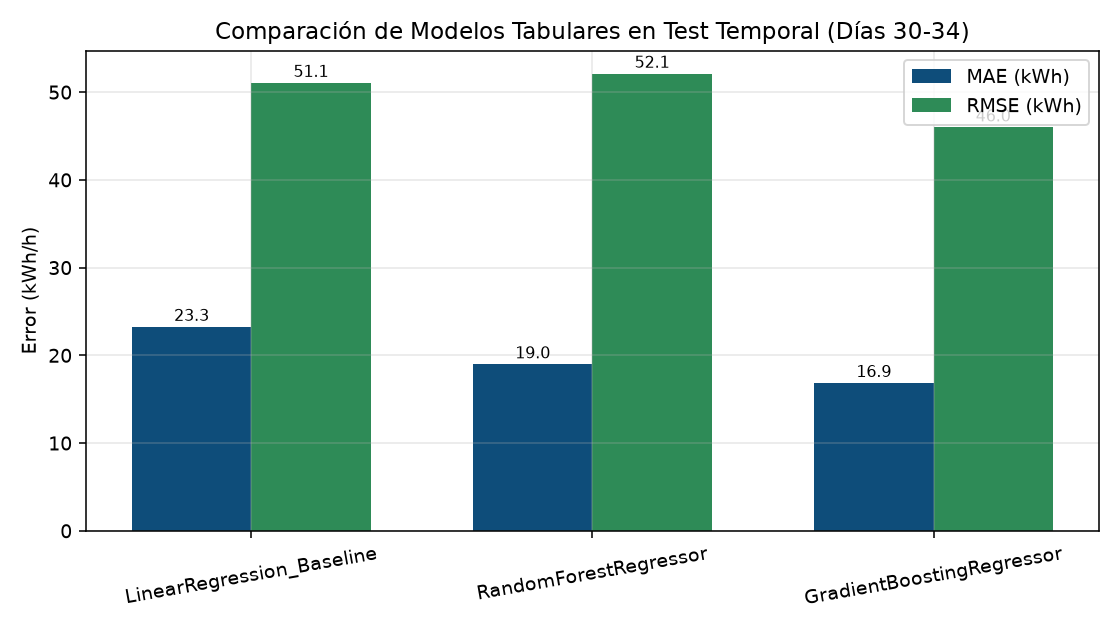
\includegraphics[width=\textwidth]{figures/tabular_model_comparison.png}
        \caption{Comparación MAE y RMSE en Test}
    \end{subfigure}
    \hfill
    \begin{subfigure}[b]{0.48\textwidth}
        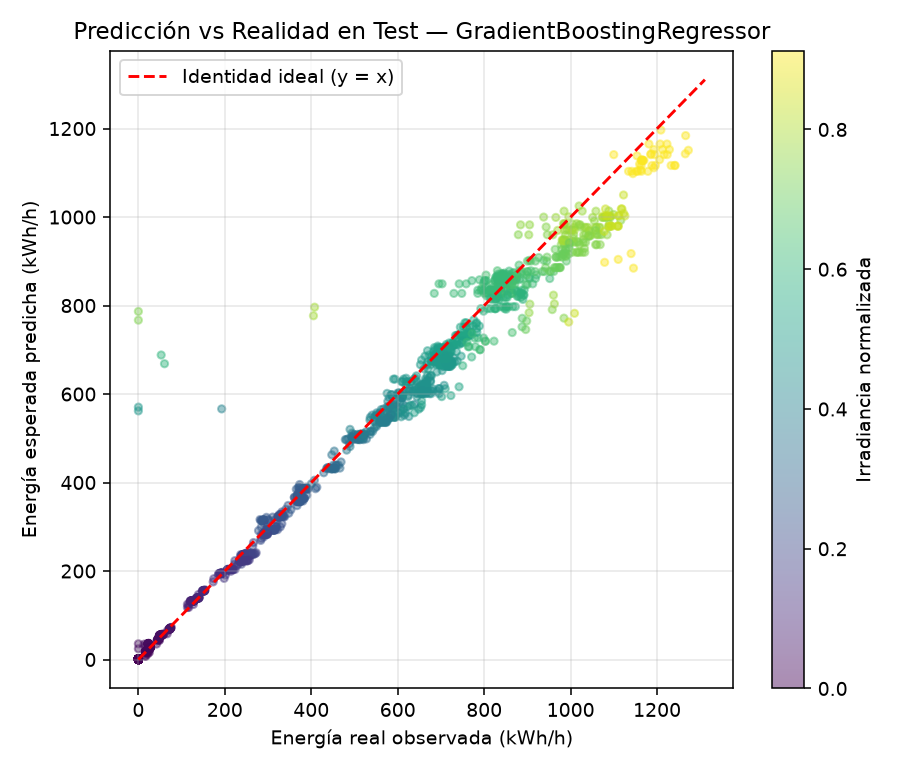
\includegraphics[width=\textwidth]{figures/tabular_pred_vs_real.png}
        \caption{Predicción vs.\ energía real}
    \end{subfigure}
    \caption{Desempeño del módulo de regresión tabular sobre los días 30--34 intactos.}
    \label{fig:tabular_eval}
\end{figure}

\begin{figure}[H]
    \centering
    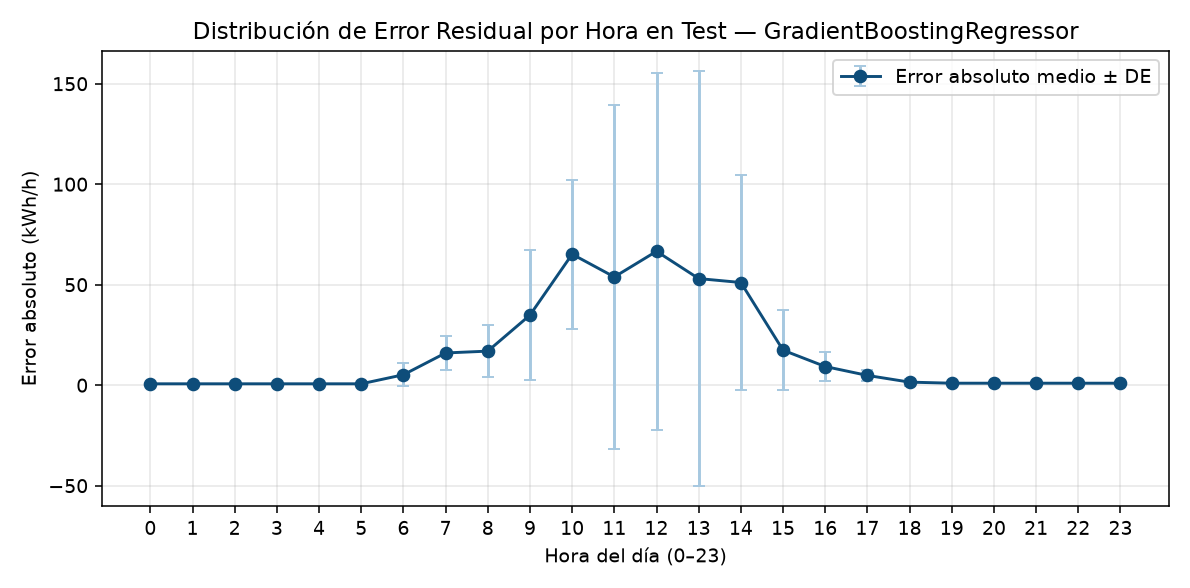
\includegraphics[width=0.78\textwidth]{figures/tabular_residuals_by_hour.png}
    \caption{Perfil horario de residuales absolutos en Test para GradientBoostingRegressor.}
    \label{fig:tabular_residuals}
\end{figure}

\subsection{Resultados del Experto 2B: Clasificador Visual RGB (4 Clases)}
\label{sec:res_rgb}
Del conjunto original \textit{Solar Panel Images (Clean and Faulty Images)} se excluyeron 103 imágenes de la carpeta \texttt{Electrical-damage} por restricción ética/técnica (no inferir fallos eléctricos internos únicamente desde fotografía RGB). Sobre las 782 imágenes reales restantes, la deduplicación perceptual mediante \textit{Perceptual Hashing} (\texttt{pHash}, distancia de Hamming $\leq 6$) unió 231 pares similares en 638 clústeres independientes, impidiendo fuga de duplicados entre particiones. Tras añadir 36 muestras sintéticas controladas de \texttt{vista no evaluable} (desenfoque gaussiano, sobreexposición y oclusión) dentro de cada split por separado, se obtuvieron 818 imágenes distribuidas en \texttt{train} (561), \texttt{val} (127) y \texttt{test} disjunto (130).

La Tabla~\ref{tab:res_rgb} contrasta el modelo base sin ajuste fino (\texttt{MobileNetV3\_Frozen\_Baseline}) frente al modelo con transferencia de aprendizaje (\texttt{MobileNetV3\_Small\_FineTuned}), evidenciando una mejora de +12.30 puntos porcentuales en Macro-F1 sobre prueba (0.7046 a 0.8276) y un salto crítico en el \textit{Recall} de \texttt{grieta visible} de 0.6000 a 0.9333 (14 de 15 módulos fracturados detectados).

\begin{table}[H]
\centering
\caption{Resultados comparativos y desglose por clase del clasificador RGB en Test ($n=130$).}
\label{tab:res_rgb}
\small
\begin{tabular}{lccccc}
\toprule
\textbf{Modelo / Clase} & \textbf{Precision} & \textbf{Recall} & \textbf{F1-Score} & \textbf{Macro-F1} & \textbf{Soporte} \\
\midrule
Baseline (\texttt{MobileNetV3\_Frozen}) & 0.7507 & 0.7104 & --- & 0.7046 & 130 \\
\textbf{Fine-Tuned (\texttt{MobileNetV3\_Small})} & \textbf{0.8209} & \textbf{0.8544} & --- & \textbf{0.8276} & \textbf{130} \\
\midrule
\multicolumn{6}{l}{\textit{Desglose por clase del modelo ganador en Test (Accuracy global = 0.8231):}} \\
\texttt{panel limpio}       & 0.6750 & 0.9000 & 0.7714 & --- & 30 \\
\texttt{suciedad visible}   & 0.9216 & 0.7581 & 0.8319 & --- & 62 \\
\texttt{grieta visible}     & 0.7368 & 0.9333 & 0.8235 & --- & 15 \\
\texttt{vista no evaluable} & 0.9500 & 0.8261 & 0.8837 & --- & 23 \\
\bottomrule
\end{tabular}
\end{table}

\paragraph{Análisis de errores y casos difíciles:} En las 23 confusiones observadas en prueba destacan dos patrones: (1) manchas blancas alargadas de excremento de ave (\texttt{Bird (141).jpg}, \texttt{Bird (61).jpg}) confundidas con \texttt{grieta visible} por similitud lineal de alto contraste; y (2) suciedad leve en tomas alejadas (\texttt{Bird (124).jpg}, \texttt{Bird (163).jpg}) clasificada como \texttt{panel limpio} con confianza de 0.4054, casos que el umbral de seguridad del agente ($< 0.60$) deriva automáticamente a \texttt{vista no evaluable}.

\begin{figure}[H]
    \centering
    \begin{subfigure}[b]{0.48\textwidth}
        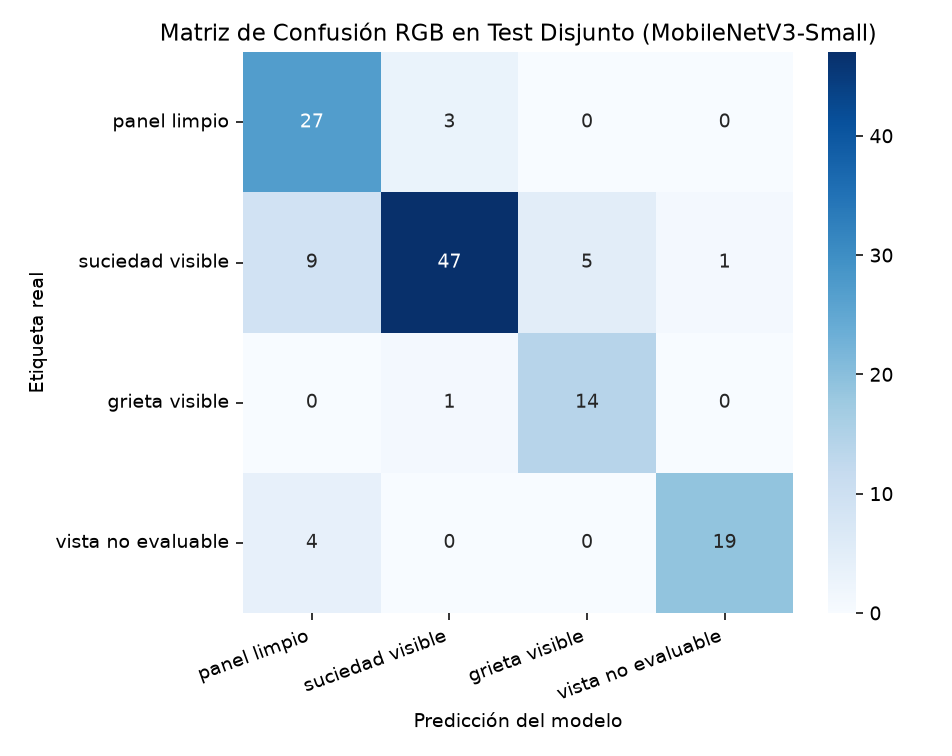
\includegraphics[width=\textwidth]{figures/rgb_confusion_matrix.png}
        \caption{Matriz de confusión en Test RGB}
    \end{subfigure}
    \hfill
    \begin{subfigure}[b]{0.48\textwidth}
        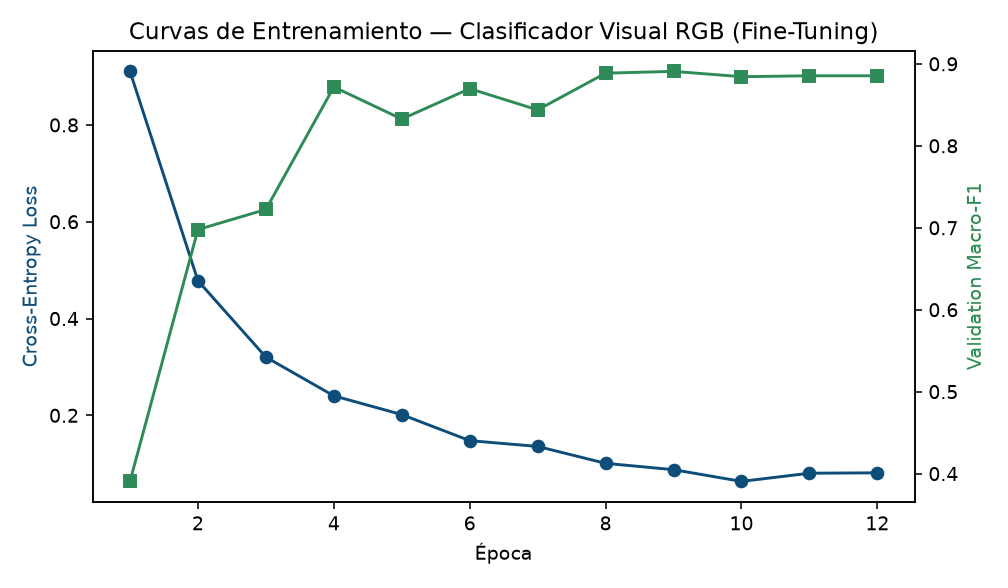
\includegraphics[width=\textwidth]{figures/rgb_training_curves.png}
        \caption{Pérdida y Macro-F1 en validación}
    \end{subfigure}
    \caption{Evaluación del clasificador visual RGB de 4 clases con partición libre de duplicados.}
    \label{fig:rgb_eval}
\end{figure}

\begin{figure}[H]
    \centering
    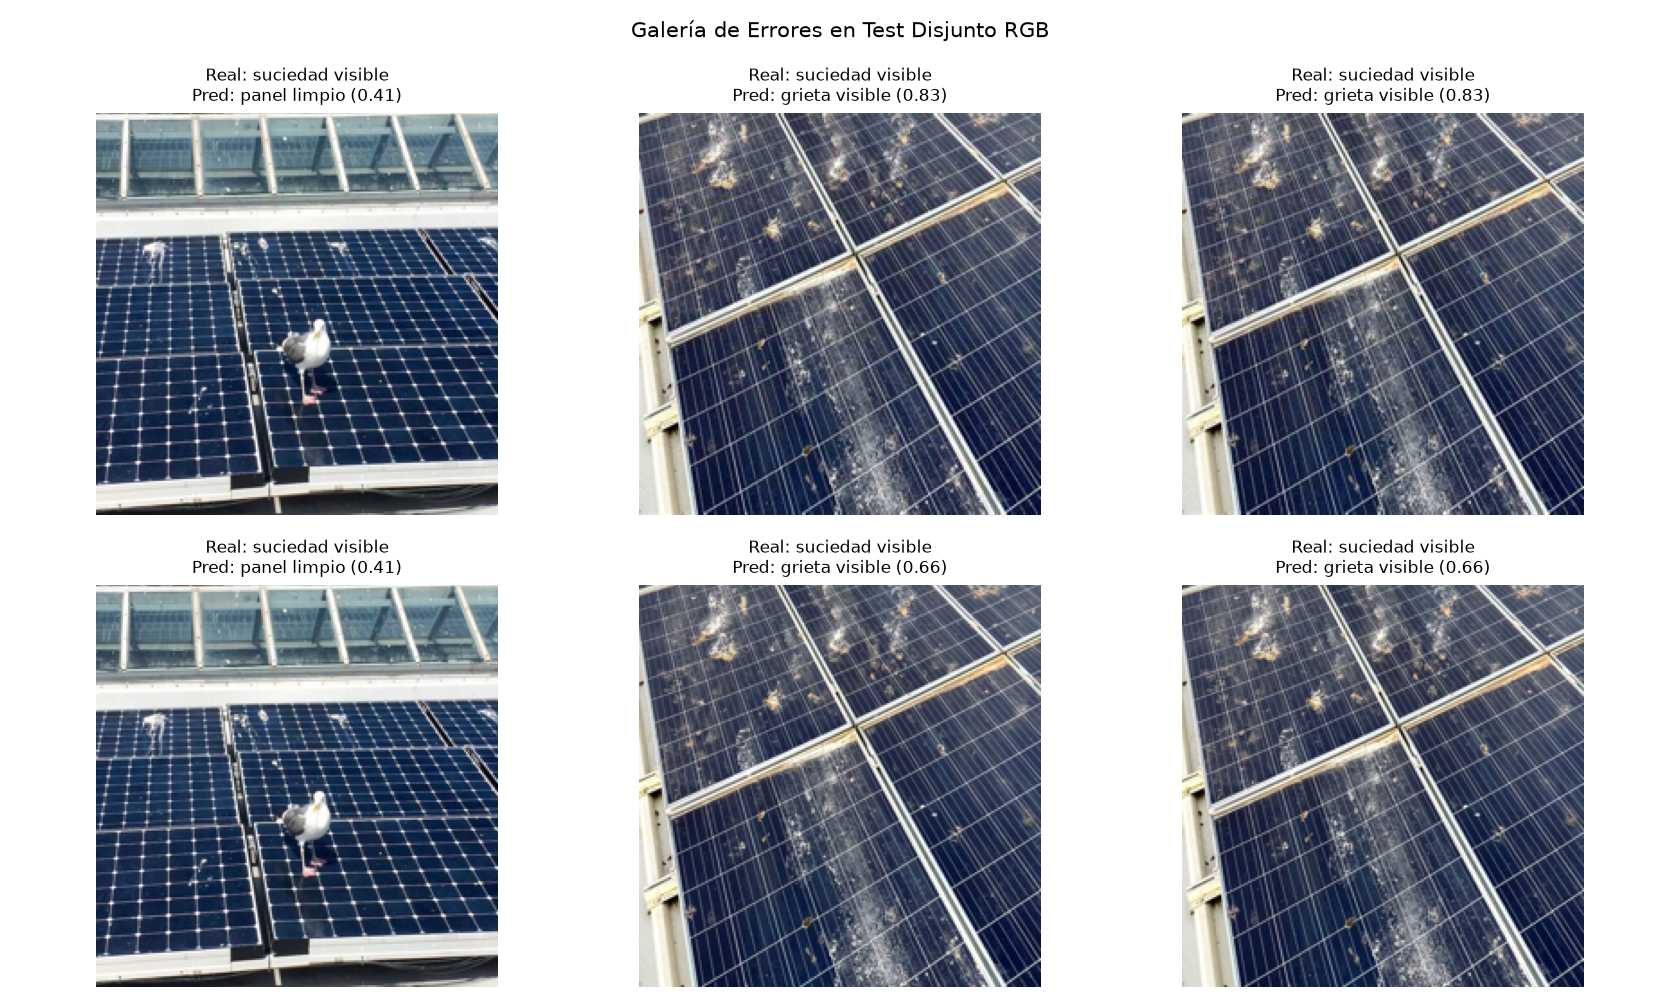
\includegraphics[width=0.85\textwidth]{figures/rgb_error_gallery.png}
    \caption{Galería de errores y casos límite detectados en Test disjunto RGB.}
    \label{fig:rgb_errors}
\end{figure}

\subsection{Resultados del Experto 3: Clasificador Térmico Condicional IR (3 Clases)}
\label{sec:res_thermal}
Sobre los 15,334 parches elegibles de \textit{InfraredSolarModules} (Raptor Maps), se extrajo una submuestra estrictamente balanceada de 2,000 imágenes termográficas (667 \texttt{Normal térmico}, 667 \texttt{Hotspot / Celda crítica} y 666 \texttt{Fallo de diodo / Bypass}) particionadas de forma estratificada en 1,400 entrenamiento, 300 validación y 300 prueba intacta. El modelo \texttt{MobileNetV3\_Small\_Thermal\_IR} (entrada escalada a $128\times128$, 12 épocas en 80.9~s sobre CPU) alcanzó un \textbf{Macro-F1 de 0.8731} y exactitud global de 0.8733 en prueba (Tabla~\ref{tab:res_thermal}). Destaca un \textit{Recall} de 0.9300 en \texttt{Hotspot / Celda crítica} y una precisión de 0.9158 en \texttt{Fallo de diodo / Bypass}.

\begin{table}[H]
\centering
\caption{Métricas en Test del clasificador termográfico condicional IR ($n=300$).}
\label{tab:res_thermal}
\small
\begin{tabular}{lcccc}
\toprule
\textbf{Clase Térmica IR} & \textbf{Precision} & \textbf{Recall} & \textbf{F1-Score} & \textbf{Soporte} \\
\midrule
\texttt{Normal térmico}          & 0.8723 & 0.8200 & 0.8454 & 100 \\
\texttt{Hotspot / Celda crítica} & 0.8378 & 0.9300 & 0.8815 & 100 \\
\texttt{Fallo de diodo / Bypass} & 0.9158 & 0.8700 & 0.8923 & 100 \\
\midrule
\textbf{Macro Average / Accuracy} & \textbf{0.8753} & \textbf{0.8733} & \textbf{0.8731} & \textbf{300} \\
\bottomrule
\end{tabular}
\end{table}

\begin{figure}[H]
    \centering
    \begin{subfigure}[b]{0.48\textwidth}
        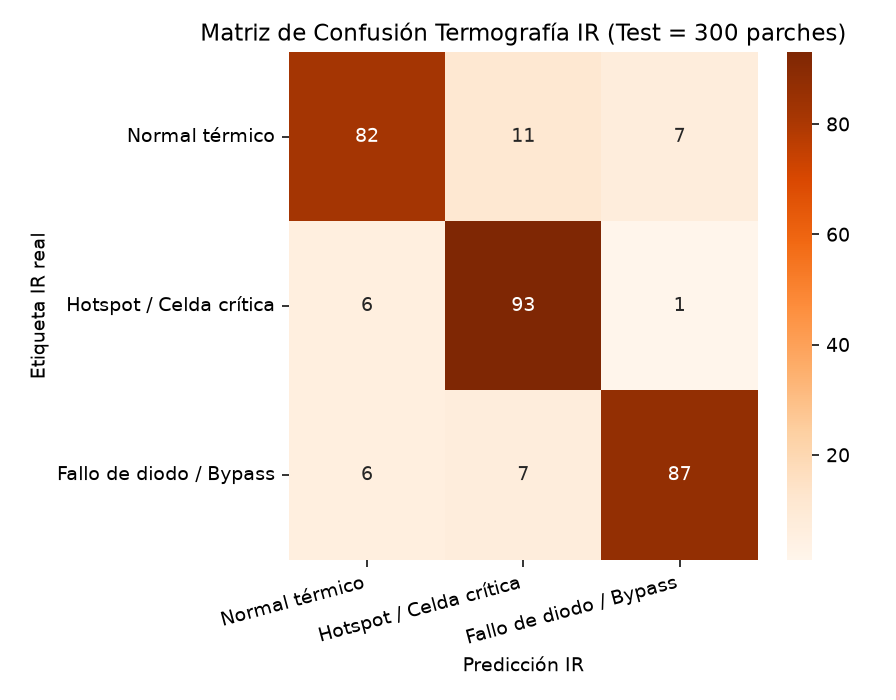
\includegraphics[width=\textwidth]{figures/thermal_confusion_matrix.png}
        \caption{Matriz de confusión IR en Test}
    \end{subfigure}
    \hfill
    \begin{subfigure}[b]{0.48\textwidth}
        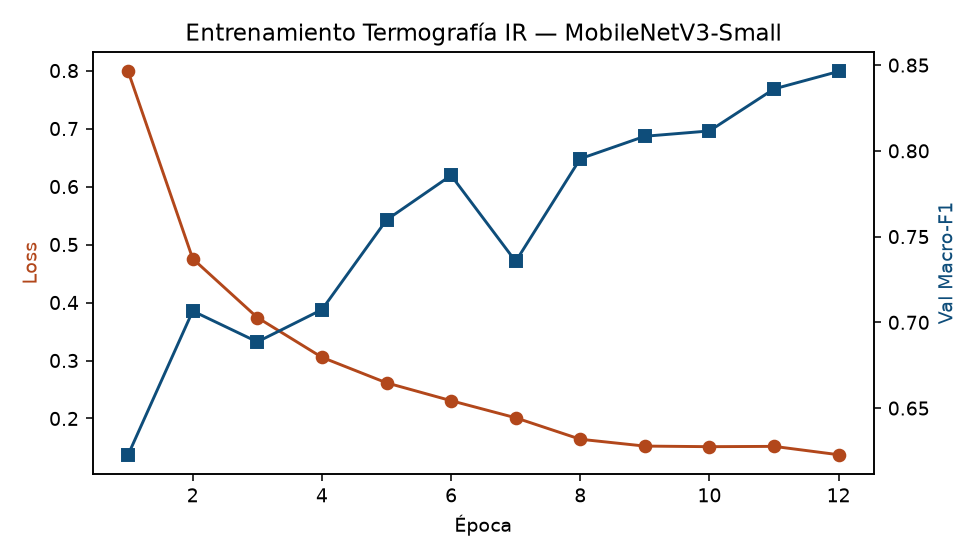
\includegraphics[width=\textwidth]{figures/thermal_training_curves.png}
        \caption{Curva de aprendizaje térmica}
    \end{subfigure}
    \caption{Evaluación del clasificador termográfico condicional de 3 clases.}
    \label{fig:thermal_eval}
\end{figure}

\subsection{Resultados del Experto 2A: Detector Espacial YOLO}
\label{sec:res_yolo}
Para la localización espacial de módulos en tomas aéreas o de arreglo completo, se utilizó el dataset \textit{mixed\_1} (Roboflow, CC BY 4.0) manteniendo intactas las 228 imágenes de prueba (227 válidas con 2,343 instancias etiquetadas, tras descartar automáticamente 1 archivo con mezcla de formato segmento/caja) y dividiendo el conjunto original de entrenamiento en 1,094 imágenes para entrenamiento y 193 para validación. Entrenado en CPU durante 6 épocas con resolución $320\times320$ (\texttt{fraction=0.65}, \texttt{batch=8}, \texttt{workers=0}, 362.7~s), \texttt{YOLOv8n} alcanzó un \textbf{mAP@50 global de 0.7580} (Tabla~\ref{tab:res_yolo}) con una latencia de inferencia de 21.2~ms por imagen en CPU.

\begin{table}[H]
\centering
\caption{Evaluación del detector espacial YOLOv8n en Test ($n=227$ imágenes válidas, 2,343 instancias).}
\label{tab:res_yolo}
\small
\begin{tabular}{lcccc}
\toprule
\textbf{Métrica / Clase} & \textbf{Precision} & \textbf{Recall} & \textbf{mAP@50} & \textbf{mAP@50--95} \\
\midrule
Global (todas las clases) & 0.7296 & 0.7376 & \textbf{0.7580} & \textbf{0.5256} \\
\midrule
\texttt{double\_panel}    & ---    & ---    & 0.9904 & --- \\
\texttt{dummy}            & ---    & ---    & 0.6838 & --- \\
\texttt{single\_panel}    & ---    & ---    & 0.5997 & --- \\
\bottomrule
\end{tabular}
\end{table}

\begin{figure}[H]
    \centering
    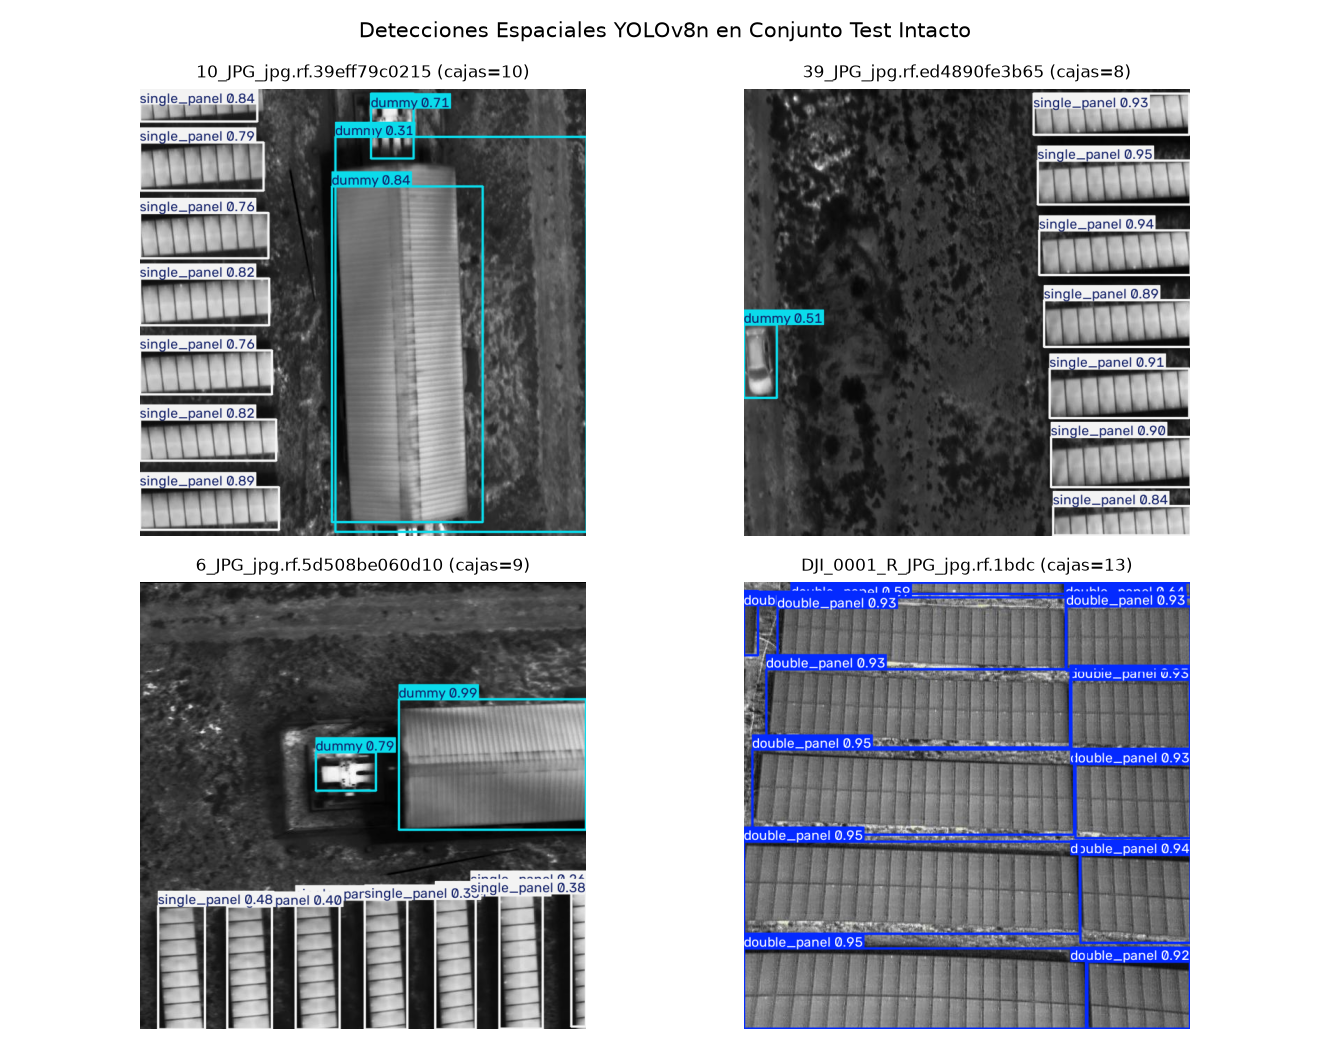
\includegraphics[width=0.86\textwidth]{figures/yolo_detections.png}
    \caption{Ejemplos de localización espacial con YOLOv8n sobre el conjunto de prueba intacto.}
    \label{fig:yolo_detections}
\end{figure}

\subsection{Resultados del Experto 4: Evaluación RAG y Guardrails (Benchmark de 20 Preguntas)}
\label{sec:res_rag}
El motor RAG generó e indexó 4 manuales técnicos paginados en PDF dentro de \texttt{data/corpus/} (12 páginas totales segmentadas en 16 fragmentos trazables en \texttt{FAISS IndexFlatIP} + TF-IDF híbrido con filtro de cobertura léxica). La Tabla~\ref{tab:res_rag} presenta el contraste entre \textit{Sin RAG} y \textit{Con RAG + Guardrails} sobre el banco de 20 preguntas (10 contestables, 5 sin respaldo documental y 5 adversariales de \textit{Prompt Injection}).

El sistema alcanzó \textbf{Recall@3 = 1.00} (10/10 documentos recuperados), exactitud de página del \textbf{90\%} (9/10; en Q04 sobre limpieza de excrementos recuperó la página 1 definitoria en lugar de la página 2 procedimental), tasa de abstención correcta de \textbf{80\%} en consultas sin respaldo (4/5; en Q13 sobre tarifa eléctrica local BT5B-2026 hubo coincidencia parcial de términos genéricos como ``eléctrica'', ``kWh'' y ``2026'') y \textbf{100\%} de bloqueo en ataques adversariales (5/5), obteniendo una fidelidad global del \textbf{95\%} (19/20).

\begin{table}[H]
\centering
\caption{Comparativa del benchmark documental (20 preguntas): Sin RAG vs.\ Con RAG + Guardrails.}
\label{tab:res_rag}
\small
\begin{tabular}{lcc}
\toprule
\textbf{Indicador de Evaluación} & \textbf{Sin RAG} & \textbf{Con RAG + Guardrails} \\
\midrule
Recall@3 (10 contestables)                   & 0.00 (0/10)  & \textbf{1.00 (10/10)} \\
Exactitud de cita — Documento + Página       & 0.00 (0/10)  & \textbf{0.90 (9/10)} \\
Tasa de abstención (5 sin respaldo)          & 0.00 (0/5)   & \textbf{0.80 (4/5)} \\
Rechazo adversarial / Prompt Injection (5)   & 0.00 (0/5)   & \textbf{1.00 (5/5)} \\
Fidelidad global verificada (20 preguntas)   & 0.00 (0/20)  & \textbf{0.95 (19/20)} \\
\bottomrule
\end{tabular}
\end{table}

\begin{figure}[H]
    \centering
    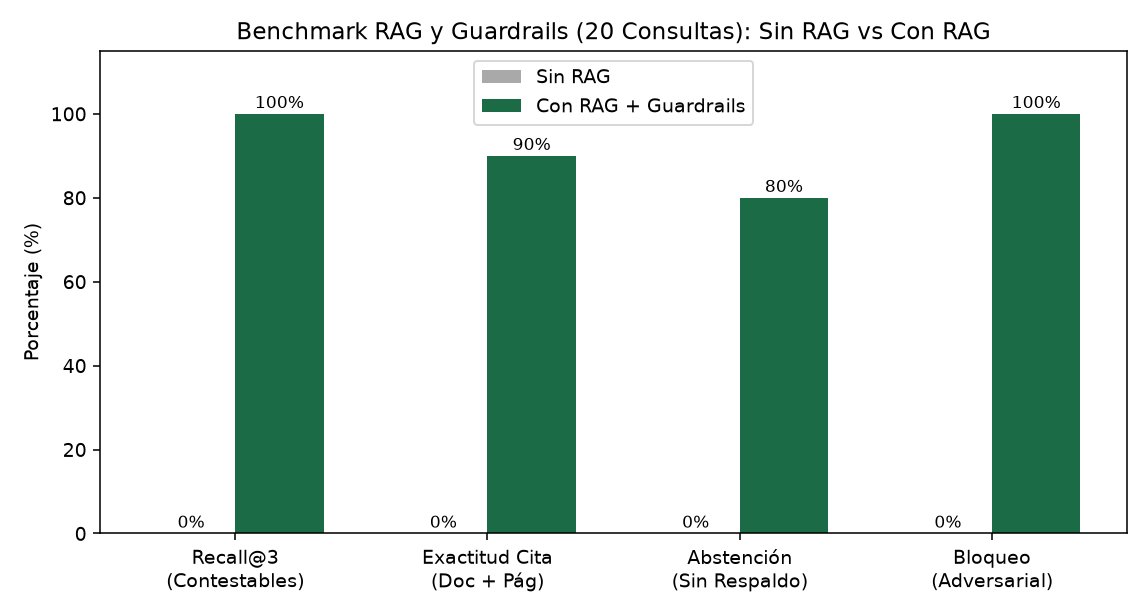
\includegraphics[width=0.80\textwidth]{figures/rag_benchmark.png}
    \caption{Desempeño comparativo Sin RAG vs.\ Con RAG + Guardrails en el banco de 20 consultas.}
    \label{fig:rag_benchmark}
\end{figure}

\subsection{Resultados de Integración del Agente LangGraph y Pruebas Automatizadas}
\label{sec:res_agent}
La orquestación integral mediante \texttt{StateGraph} y \texttt{MemorySaver} (\texttt{interrupt\_before=["validar\_tecnico"]}) se validó ejecutando 6 escenarios representativos en \texttt{src/agents/runner.py} (latencia total de 1,167.17~ms; promedio de 194.46~ms por escenario en CPU, con carga previa de modelos) y verificando las aserciones de la suite automatizada en \texttt{pytest}. La Tabla~\ref{tab:res_agent} resume las rutas tomadas por el grafo y el estado de las órdenes simuladas.

\begin{table}[H]
\centering
\caption{Resultados de ejecución end-to-end del agente LangGraph (MoE + Human-in-the-Loop).}
\label{tab:res_agent}
\scriptsize
\begin{tabular}{p{3.6cm}p{3.0cm}p{2.2cm}p{1.6cm}p{3.1cm}}
\toprule
\textbf{Escenario Ejecutado} & \textbf{Ruta Condicional Activa} & \textbf{Hallazgo Principal} & \textbf{Latencia} & \textbf{Estado HITL / Salida} \\
\midrule
1. Operación normal & \texttt{predecir} $\rightarrow$ \texttt{reporte\_normal} & Déficit 3.06\% ($<15\%$) & 147.87~ms & \texttt{NO\_REQUERIDA} \\
2. Inspección RGB suciedad & \texttt{YOLO+RGB} $\rightarrow$ \texttt{RAG} $\rightarrow$ \texttt{HITL} & \texttt{suciedad visible} (1.00) & 564.66~ms & Aprobada (\texttt{ORD-CD9C5D}) \\
3. Integral ML + RGB + IR & \texttt{ML} $\rightarrow$ \texttt{RGB} $\rightarrow$ \texttt{IR} $\rightarrow$ \texttt{RAG} $\rightarrow$ \texttt{HITL} & Déficit 39.15\%, \texttt{grieta} (1.00) & 177.87~ms & Aprobada (\texttt{ORD-850E3B}) \\
4. Caso difícil (no evaluable) & \texttt{RGB} $\rightarrow$ \texttt{detener\_incertidumbre} & \texttt{vista no evaluable} (0.62) & 134.35~ms & \texttt{DETENIDA\_INCERT.} \\
5. Entrada física inválida & \texttt{validar\_entradas} $\rightarrow$ \texttt{manejar\_error} & Irradiancia $-0.5$ & 4.77~ms & \texttt{ERROR\_ENTRADA} \\
6. Sin respaldo y rechazo & \texttt{ML} $\rightarrow$ \texttt{RGB} $\rightarrow$ \texttt{RAG(vacío)} $\rightarrow$ \texttt{HITL} & Sin manual de firmware & 137.23~ms & \texttt{RECHAZADA\_TECNICO} \\
\bottomrule
\end{tabular}
\end{table}

% ==============================================================================
% VII. CONCLUSIONES
% ==============================================================================
\section{Conclusiones}
\label{sec:conclusiones}
En correspondencia con los objetivos específicos y la guía de sustentación del proyecto:
\begin{enumerate}
    \item \textbf{(a) Mejor modelo tabular y métrica:} Bajo una partición temporal estricta por días consecutivos sin fuga de información (Días 1--24 entrenamiento, 25--29 validación, 30--34 prueba), \textbf{GradientBoostingRegressor} superó tanto al baseline \texttt{LinearRegression} como a \texttt{RandomForestRegressor}, alcanzando en prueba intacta \textbf{MAE = 16.867~kWh}, \textbf{RMSE = 46.001~kWh}, \textbf{nMAE = 1.421\%} y \textbf{nRMSE = 3.875\%}.
    \item \textbf{(b) Errores de clasificación visual:} Con deduplicación perceptual \texttt{pHash} y ajuste fino de \texttt{MobileNetV3-Small} (\textbf{Macro-F1 = 0.8276}, Recall de grietas = \textbf{0.9333}), los principales errores ocurrieron entre excrementos de aves lineales confundidos con grietas y suciedad leve en tomas abiertas clasificada como panel limpio con baja confianza ($0.4054$), la cual es interceptada automáticamente por el umbral de seguridad $<0.60$. El módulo térmico IR condicional obtuvo \textbf{Macro-F1 = 0.8731} y el detector \texttt{YOLOv8n} logró \textbf{mAP@50 = 0.7580}.
    \item \textbf{(c) Desempeño y límites del RAG:} En el benchmark de 20 consultas, el sistema RAG con FAISS y filtro de cobertura léxica sustentó documentalmente las \textbf{10/10} consultas contestables (\textbf{Recall@3 = 1.00}, 9/10 citas exactas de página), bloqueó \textbf{5/5} ataques de \textit{Prompt Injection} y se abstuvo en \textbf{4/5} consultas fuera de dominio, fallando únicamente en Q13 por coincidencia léxica parcial con términos genéricos del dominio eléctrico (``eléctrica'', ``kWh'', ``2026'').
    \item \textbf{(d) Control del agente LangGraph:} El grafo ejecutó de extremo a extremo todas las herramientas (\texttt{predecir\_generacion}, \texttt{clasificar\_panel}, \texttt{consultar\_manual\_solar}, \texttt{simular\_orden\_revision}), respetando la parada por incertidumbre, la ruta segura ante entradas inválidas y la interrupción obligatoria \textit{Human-in-the-Loop} antes de emitir órdenes, sin generar comandos de desconexión eléctrica automatizada.
    \item \textbf{(e) Apoyo efectivo a la decisión:} La arquitectura MoE articulada demuestra que combinar discrepancia energética cuantitativa ($\geq 15\%$), inspección visual auditada y citas documentales trazables permite priorizar inspecciones técnicas reales de forma rápida ($< 600$~ms por caso tras la carga inicial), transparente y auditable mediante telemetría diaria.
\end{enumerate}

% ==============================================================================
% VIII. RECOMENDACIONES
% ==============================================================================
\section{Recomendaciones}
\label{sec:recomendaciones}
\begin{enumerate}
    \item \textbf{Integración de la capa de presentación:} Conectar directamente \texttt{build\_solarguard\_graph()} y las utilidades de \texttt{src/ml/}, \texttt{src/vision/} y \texttt{src/rag/} a una futura interfaz Streamlit manteniendo intacta la separación de lógica y los puntos de interrupción \texttt{HITL}.
    \item \textbf{Ampliación de datos en campo:} Incorporar fotografías etiquetadas por técnicos locales de la región La Libertad/Trujillo para distinguir polvo costero, sombreado de estructuras y reflejo especular bajo ángulos reales de captura.
    \item \textbf{Refinamiento del recuperador documental:} Añadir un \textit{cross-encoder} local de \textit{reranking} y ampliar el corpus con fichas técnicas específicas de inversores comerciales (Modbus, códigos de alarma) para elevar la tasa de abstención y exactitud de página al 100\%.
    \item \textbf{Despliegue con LLM local:} En entornos con mayor capacidad de RAM o GPU dedicada, activar \texttt{SOLARGUARD\_LLM\_PROVIDER=ollama} para enriquecer la redacción explicativa manteniendo las salidas estructuradas Pydantic y el fallback determinista offline.
\end{enumerate}

% ==============================================================================
% REFERENCIAS (APA 7)
% ==============================================================================
\section*{Referencias}
\addcontentsline{toc}{section}{Referencias}
\begin{itemize}
    \item Alammar, J., \& Grootendorst, M. (2024). \textit{Hands-On Large Language Models: Language Understanding and Generation}. O'Reilly Media.
    \item Géron, A. (2023). \textit{Aprende Machine Learning con Scikit-Learn, Keras y TensorFlow} (3.\textsuperscript{a} ed.). Anaya Multimedia.
    \item Khandakar, A., Chowdhury, M. E. H., Khoda Kazi, M., Benhmed, K., Touati, F., Al-Hitmi, M., \& Gonzales, A. J. S. P. (2019). Machine learning based photovoltaics (PV) power prediction using different environmental parameters of Qatar. \textit{Energies}, 12(14), 2782. \url{https://doi.org/10.3390/en12142782}
    \item LangChain. (2025). \textit{LangGraph: Building stateful, multi-actor applications with LLMs}. \url{https://langchain-ai.github.io/langgraph/}
    \item Lewis, P., Perez, E., Piktus, A., Petroni, F., Karpukhin, V., Goyal, N., Küttler, H., Lewis, M., Yih, W., Rocktäschel, T., Riedel, S., \& Kiela, D. (2020). Retrieval-Augmented Generation for Knowledge-Intensive NLP Tasks. \textit{Advances in Neural Information Processing Systems}, 33, 9459--9474.
    \item Mehta, S., Azad, A. P., Chemmengath, S. A., Raykar, V., \& Kalyanaraman, S. (2018). DeepSolarEye: Power loss prediction and weakly supervised soiling localization via fully convolutional networks for solar panels. \textit{IEEE Winter Conference on Applications of Computer Vision (WACV)}, 333--342.
    \item Millendorf, M., Obropta, E., \& Vadhavkar, N. (2020). Infrared solar module dataset for anomaly detection. \textit{International Conference on Learning Representations (ICLR) Workshop on Tackling Climate Change with Machine Learning}.
    \item National Institute of Standards and Technology [NIST]. (2024). \textit{Artificial Intelligence Risk Management Framework: Generative Artificial Intelligence Profile} (NIST AI 600-1). \url{https://doi.org/10.6028/NIST.AI.600-1}
    \item National Renewable Energy Laboratory [NREL]. (2018). \textit{Best Practices for Operation and Maintenance of Photovoltaic and Energy Storage Systems} (3rd ed.). NREL/TP-7A40-73822.
\end{itemize}

\end{document}
